
The results from the given simulations are summarized through the number of
collisions, the total length of the solution trajectories, and the number of
branches added to each search tree. These performance measures are shown in
\cref{table:results}, \cref{table:results-length}
and \cref{table:results-iterations} respectivly. For each column total of
hundred simulation is performed. In the first table a count of how many of the
simulations runs that resulted in a collision is given, while in the latter two tables an
average of the hundred simulation runs are given.


\begin{table}[!t]
  \centering
  \begin{IEEEeqnarraybox}[\IEEEeqnarraystrutmode \IEEEeqnarraystrutsizeadd{2pt}{1pt}]{v/c/v/c/v/c/v/c/v}
    \IEEEeqnarrayrulerow\\
    &\mbox{Number of Collisions}&&w=0 \, m/s&&w=3 \, m/s&& w=6 \, m/s\\
    \IEEEeqnarraydblrulerow\\
    \IEEEeqnarrayseprow[3pt]\\
    &\mathrm{\rrtfunnel}&& 0 && 0 && 4 &\IEEEeqnarraystrutsize{0pt}{0pt}\\
    \IEEEeqnarrayseprow[3pt]\\
    %%
    \IEEEeqnarrayrulerow\\
    \IEEEeqnarrayseprow[3pt]\\
    &\mathrm{Benchmark}&& 0 && 6 && 10 &\IEEEeqnarraystrutsize{0pt}{0pt}\\
    \IEEEeqnarrayseprow[3pt]\\
    \IEEEeqnarrayrulerow
    % %%
    % \vspace{2em}\\
    % %%
    % \IEEEeqnarrayrulerow\\
    % \IEEEeqnarrayrulerow\\
    % &\mbox{Number of Iterations}&&w=0 \, m/s&&w=3 \, m/s&& w=6 \, m/s\\
    % \IEEEeqnarraydblrulerow\\
    % \IEEEeqnarrayseprow[3pt]\\
    % &\mathrm{\rrtfunnel}&& 447.646 && 190.713 && 213.638 &\IEEEeqnarraystrutsize{0pt}{0pt}\\
    % \IEEEeqnarrayseprow[3pt]\\
    % %%
    % \IEEEeqnarrayrulerow\\
    % \IEEEeqnarrayseprow[3pt]\\
    % &\mathrm{Benchmark}&& 29.120 && 52.768 && 33.936 &\IEEEeqnarraystrutsize{0pt}{0pt}\\
    % \IEEEeqnarrayseprow[3pt]\\
    % \IEEEeqnarrayrulerow
    % %%
    % \vspace{2em}\\
    % %%
    % \IEEEeqnarrayrulerow\\
    % \IEEEeqnarrayrulerow\\
    % &\mbox{Solution Trajectory's Length}&&w=0 \, m/s&&w=3 \, m/s&& w=6 \, m/s\\
    % \IEEEeqnarraydblrulerow\\
    % \IEEEeqnarrayseprow[3pt]\\
    % &\mathrm{\rrtfunnel}&& 1.506 && 3.418 && 4.754 &\IEEEeqnarraystrutsize{0pt}{0pt}\\
    % \IEEEeqnarrayseprow[3pt]\\
    % %%
    % \IEEEeqnarrayrulerow\\
    % \IEEEeqnarrayseprow[3pt]\\
    % &\mathrm{Benchmark}&& 3.582 && 4.162 && 3.174 &\IEEEeqnarraystrutsize{0pt}{0pt}\\
    % \IEEEeqnarrayseprow[3pt]\\
    % \IEEEeqnarrayrulerow
  \end{IEEEeqnarraybox}
  \caption{The total number of collisions for each algorithm over a total of 100 simulation runs, with three different values for
    the cross-wind (w).} \label{table:results}
\end{table}

\begin{table}[!t]
  \centering
  \begin{IEEEeqnarraybox}[\IEEEeqnarraystrutmode \IEEEeqnarraystrutsizeadd{2pt}{1pt}]{v/c/v/c/v/c/v/c/v}
    \IEEEeqnarrayrulerow\\
    &\mbox{Solution Trajectory's Length}&&w=0 \, m/s&&w=3 \, m/s&& w=6 \, m/s\\
    \IEEEeqnarraydblrulerow\\
    \IEEEeqnarrayseprow[3pt]\\
    &\mathrm{\rrtfunnel}&& 1.506 && 3.418 && 4.754 &\IEEEeqnarraystrutsize{0pt}{0pt}\\
    \IEEEeqnarrayseprow[3pt]\\
    %% 
    \IEEEeqnarrayrulerow\\
    \IEEEeqnarrayseprow[3pt]\\
    &\mathrm{Benchmark}&& 3.582 && 4.162 && 3.174 &\IEEEeqnarraystrutsize{0pt}{0pt}\\
    \IEEEeqnarrayseprow[3pt]\\
    \IEEEeqnarrayrulerow
  \end{IEEEeqnarraybox}
  \caption{The total length of the solutions found for each algorithm over a total of 100 simulation runs, with three different values for the cross-wind (w).} \label{table:results-length}
\end{table}

\begin{table}[!t]
  \centering
  \begin{IEEEeqnarraybox}[\IEEEeqnarraystrutmode \IEEEeqnarraystrutsizeadd{2pt}{1pt}]{v/c/v/c/v/c/v/c/v}
    \IEEEeqnarrayrulerow\\
    &\mbox{Number of Iterations}&&w=0 \, m/s&&w=3 \, m/s&& w=6 \, m/s\\
    \IEEEeqnarraydblrulerow\\
    \IEEEeqnarrayseprow[3pt]\\
    &\mathrm{\rrtfunnel}&& 447.646 && 190.713 && 213.638 &\IEEEeqnarraystrutsize{0pt}{0pt}\\
    \IEEEeqnarrayseprow[3pt]\\
    %% 
    \IEEEeqnarrayrulerow\\
    \IEEEeqnarrayseprow[3pt]\\
    &\mathrm{Benchmark}&& 29.120 && 52.768 && 33.936 &\IEEEeqnarraystrutsize{0pt}{0pt}\\
    \IEEEeqnarrayseprow[3pt]\\
    \IEEEeqnarrayrulerow
  \end{IEEEeqnarraybox}
  \caption{The total number of iterations for each algorithm over a total of 100 simulation runs, with three different values for the cross-wind (w).} \label{table:results-iterations}
\end{table}


A plot of the Lyapunov
values for a simulation run can be seen in \cref{fig:lyapunov-values}.

\begin{figure}[!t]
  \centering
  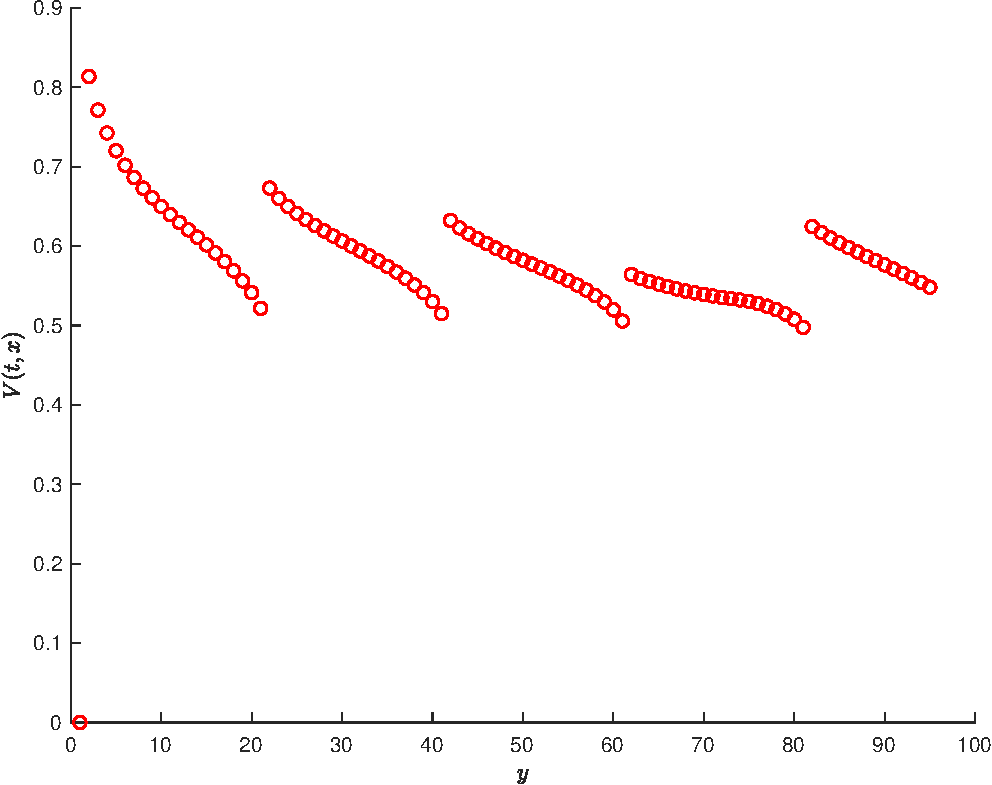
\includegraphics[width=.8\columnwidth]{figures/experiments/lyapunov-values-simulation-run}
  \caption[A plot of the Lyapunov values for an experiment]{The plot of the Lyapunov values for a simulation run at the sampling
    times \(t_k\).}
  \label{fig:lyapunov-values}
\end{figure}

